\documentclass[fleqn,11pt]{SelfArx} 
%\setlength{\fboxrule}{0.75pt} % Width of the border around the abstract
\definecolor{color1}{RGB}{0,0,100} % Color of the article title and sections
\definecolor{color2}{RGB}{0,0,0} % Color of the boxes behind the abstract and headings
\usepackage{hyperref} % Required for hyperlinks
\hypersetup{hidelinks,colorlinks,breaklinks=true,urlcolor=color2,citecolor=color1,linkcolor=color1,bookmarksopen=false,pdftitle={Title},pdfauthor={Author}}

%----------------------------------------------------------------------------------------
%	ARTICLE INFORMATION
%----------------------------------------------------------------------------------------
\PaperTitle{Nuclear receptor variation in mice} % Article title

\Authors{Beratis, Alexander, Iacob, Diana, Boyanova, Dr. Desislava\textsuperscript{1}, Mewes, Prof. Dr. Hans-Werner\textsuperscript{1}} % Authors
\affiliation{\textsuperscript{1}\textit{Institute of Bioinformatics and Systems Biology, Helmholtz Zentrum M�nchen, German Research Center for Environmental Health,}} % Author affiliation

\Keywords{Nuclear receptors --- SNPs --- Gene variation} % Keywords
\newcommand{\keywordname}{Keywords} % Defines the keywords heading name

%----------------------------------------------------------------------------------------
%	ABSTRACT
%----------------------------------------------------------------------------------------

\Abstract{\textit{
Nuclear receptors (NRs) are a large family of ligand-activated transcription factors, that bind directly to DNA to regulate the expression of target genes. They regulate critical functions in cell control, inflammation, fibrosis and tumor formation and are involved in metabolism, development and reproduction. Nuclear receptors influence the metabolism and signalling processes in the cells by changing the expression of target genes and are associated with numerous pathologies such as cancer, cardiovascular disease, and reproductive abnormalities. This paper presents the investigative results of knockout phenotypes and genetic variation for mouse NRs. Based on an assembly of all known mouse SNPs in the mouse NR genes, the phenotype information for genetic knockouts and genetic variation data was compiled from public databases. Knockout phenotypes were extracted from the Mouse Genome Informatics (MGI) database, while the Mouse Phenome Database (MPD) provides SNPs from various mouse strains, which can be correlated with extreme phenotypes measured in these mouse strains. The goal of this analysis is to find NR-associated SNPs in mice that influence changes in biological parameters such as body weight, body fat and other phenotypic traits. Furthermore, these findings will be coupled to phenotypes observed in mice with a targeted or spontaneous mutation of the nuclear receptor and thus provide additional indication for a putative functionality of the investigated SNPs.}}

%----------------------------------------------------------------------------------------

\begin{document}

\flushbottom % Makes all text pages the same height
\maketitle % Print the title and abstract box
\thispagestyle{empty} % Removes page numbering from the first page

%----------------------------------------------------------------------------------------
%	ARTICLE CONTENTS
%----------------------------------------------------------------------------------------

\section*{Introduction} % The \section*{} command stops section numbering

Looking across the evolutionary patterns between mouse and human, numerous research experiments and gene regulation studies have shown striking similarities regarding certain processes and systems in the two organisms. The mouse presents up to 95\% genome similarity to humans and is thus often being used as a model organism when investigating anatomical, physiological or genetical markers in humans. Practically, mice are small, have an accelerated life cycle and represent a cost-effective alternative to genetic research and drug development for human diseases. Also, the majority of the genes responsible for complex diseases are shared between mice and humans, enhancing the chances of successfully identifying patterns in mice which would reveal human disease phenotypes~\cite{intro1}.
~~~~~~~\\
~~~~~~~\\  
This paper makes use of the publicly available data in the Mouse Genome Informatics database and Mouse Phenome Database, respectively, in order to highlight changes in various biological parameters in mice under the influence of the NR-associated SNPs. Furthermore, these findings can be mapped to genotype - phenotype associations in humans, for studying the human biology and disease.

%------------------------------------------------

\section{Methods}

Both the process of consolidating a genotype - phenotype map, as well as the subsequent analysis of extreme phenotypes observed in mice rely on four biological elements: mouse strains, gene names / symbols, nuclear receptors, SNPs. The correlation between the position of a nuclear receptor and various SNPs on a gene can result in a specific phenotype. Due to increased specificity rate of the phenotype associated with a particular nuclear receptor, different NR and SNPs associations will result in different phenotypes for the same gene. Similarly, diverging mouse strains present non-identical phenotypes for the genetic parameters.  

\subsection{Mouse nuclear receptors}

The analysis presented in this paper was based upon a dataset consisting of the 49 nuclear receptors of mouse~\cite{proteomic} and their associated genes (242 unique gene Ids, 49 gene names / symbols); for a full list of gene names, see Appendix~\ref{an:appendix}). The gene names were further on used to compile additional information regarding the position, associated SNPs and phenotypes for the nuclear receptors in mice.

\subsection{MGI - Mouse Genome Informatics}

Mouse Genome Informatics\footnote{\url{http://www.informatics.jax.org/}, \today}~\cite{mgi} is a free, online database for the laboratory mouse and provides access to information about integrated genetics and associations between specific phenotypes and their corresponding alleles. It contains over 24000 genes and their protein sequences and approximately 48000 genotypes and phenotype annotations. For this research, the MGI database was solely used for building a connection between the nuclear receptor genes in the mouse and the associated phenotypes dependent on miscellaneous strains. 

\subsection{MPD - Mouse Phenome Database}

Mouse Phenome Database\footnote{\url{http://phenome.jax.org/}, \today}~\cite{mpd} includes annotations of measured data on the laboratory mouse strains and populations, as well as SNPs and phenotypes of the examined strains. More than 1330 strains were examined, providing annotations for over 3500 phenotype and 1.8 billion genotypes. 
~~~~~~~\\
~~~~~~~\\  
The MPD database is more detailed and comprehensive than the MGI, so that the phenotypes found in MGI can be traced back to MPD. However, the MPD strictly associates individual phenotypes to their corresponding strain, posing difficulties in the mapping process between the mouse nuclear receptors and the MGI data. 

%------------------------------------------------

\section{Database}

Since annotation from multiple public databases and internal data were used, there was a need to design and implement a database supporting the research. The database structure thereby presents 7 tables and aims to facilitate the processes of gathering, parsing and statistical analysis of the nuclear receptors data, as well as to allow for a clear mapping between the nuclear receptor genes and the phenotypes and SNPs associated with them. 
The main challenge was to establish a connection between the MGI, MPD and UCSC tables. Therefore, there are 2 tables containing information from the MGI, 3 tables for MPD, 1 USCS table and the core table:
\begin{itemize}
\item \textbf{nr\_mapping} - core table, which contains the associations between the 49 nuclear receptors in the mouse and their corresponding gene names. 
\item \textbf{mgi} - contains the MGI gene annotations (MGI gene id, type, attributes, transmission etc.). 
\item \textbf{mgi\_phenotypes} - stores phenotypic information in association with MGI genes; more than one phenotype can be associated with a specific gene.
\item \textbf{mpd\_snp} - contains the MPD SNP-annotations in correlation with the nuclear receptor genes. 
\item \textbf{ucsc} - contains a more detailed overview on the MPD mutations from \textit{mpd\_snp} 
\item \textbf{mpd\_strains} - contains the MPD strain annotations (MPD strain id, sex, number of mice, Z-score etc.)
\item \textbf{mpd\_phenotypes} - stores phenotypic information in association with MPD strains; more than one phenotype can be associated with a specific strain.
\end{itemize} 
~~~~~~~\\  
\begin{figure}[H]
	\centering
	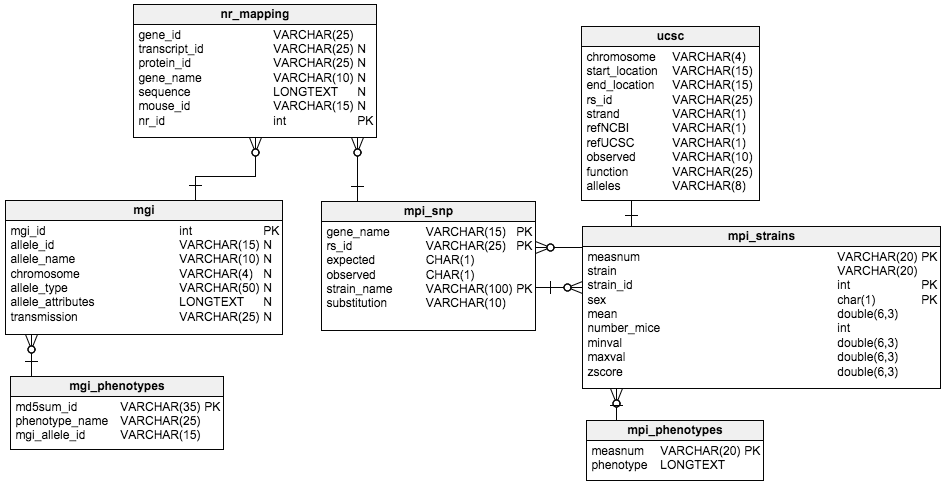
\includegraphics[width=\linewidth]{pics/db.png}
	\captionsetup{margin=12pt,format=plain,font=footnotesize,labelfont=bf}
 	\caption{\footnotesize{\textbf{Database}. 
	~~~~~~~\\
	Database scheme for the 49 nuclear receptors with information about MGI, MPI and UCSC.}}
	\label{fig:mgi_pheotypes_distribution}
\end{figure}
%------------------------------------------------

\section{Results}
The goal hereby was to visualise the most important phenotypes associated with the 49 nuclear receptors in the mouse. In this regard, the phenotypic and genomic data from the MGI and MPD was compared and analysed. All graphics were generated using the R package\footnote{\url{www.r-project.org/}, \today}.

\subsection{MGI Statistics}

\begin{figure}[H]
	\centering
	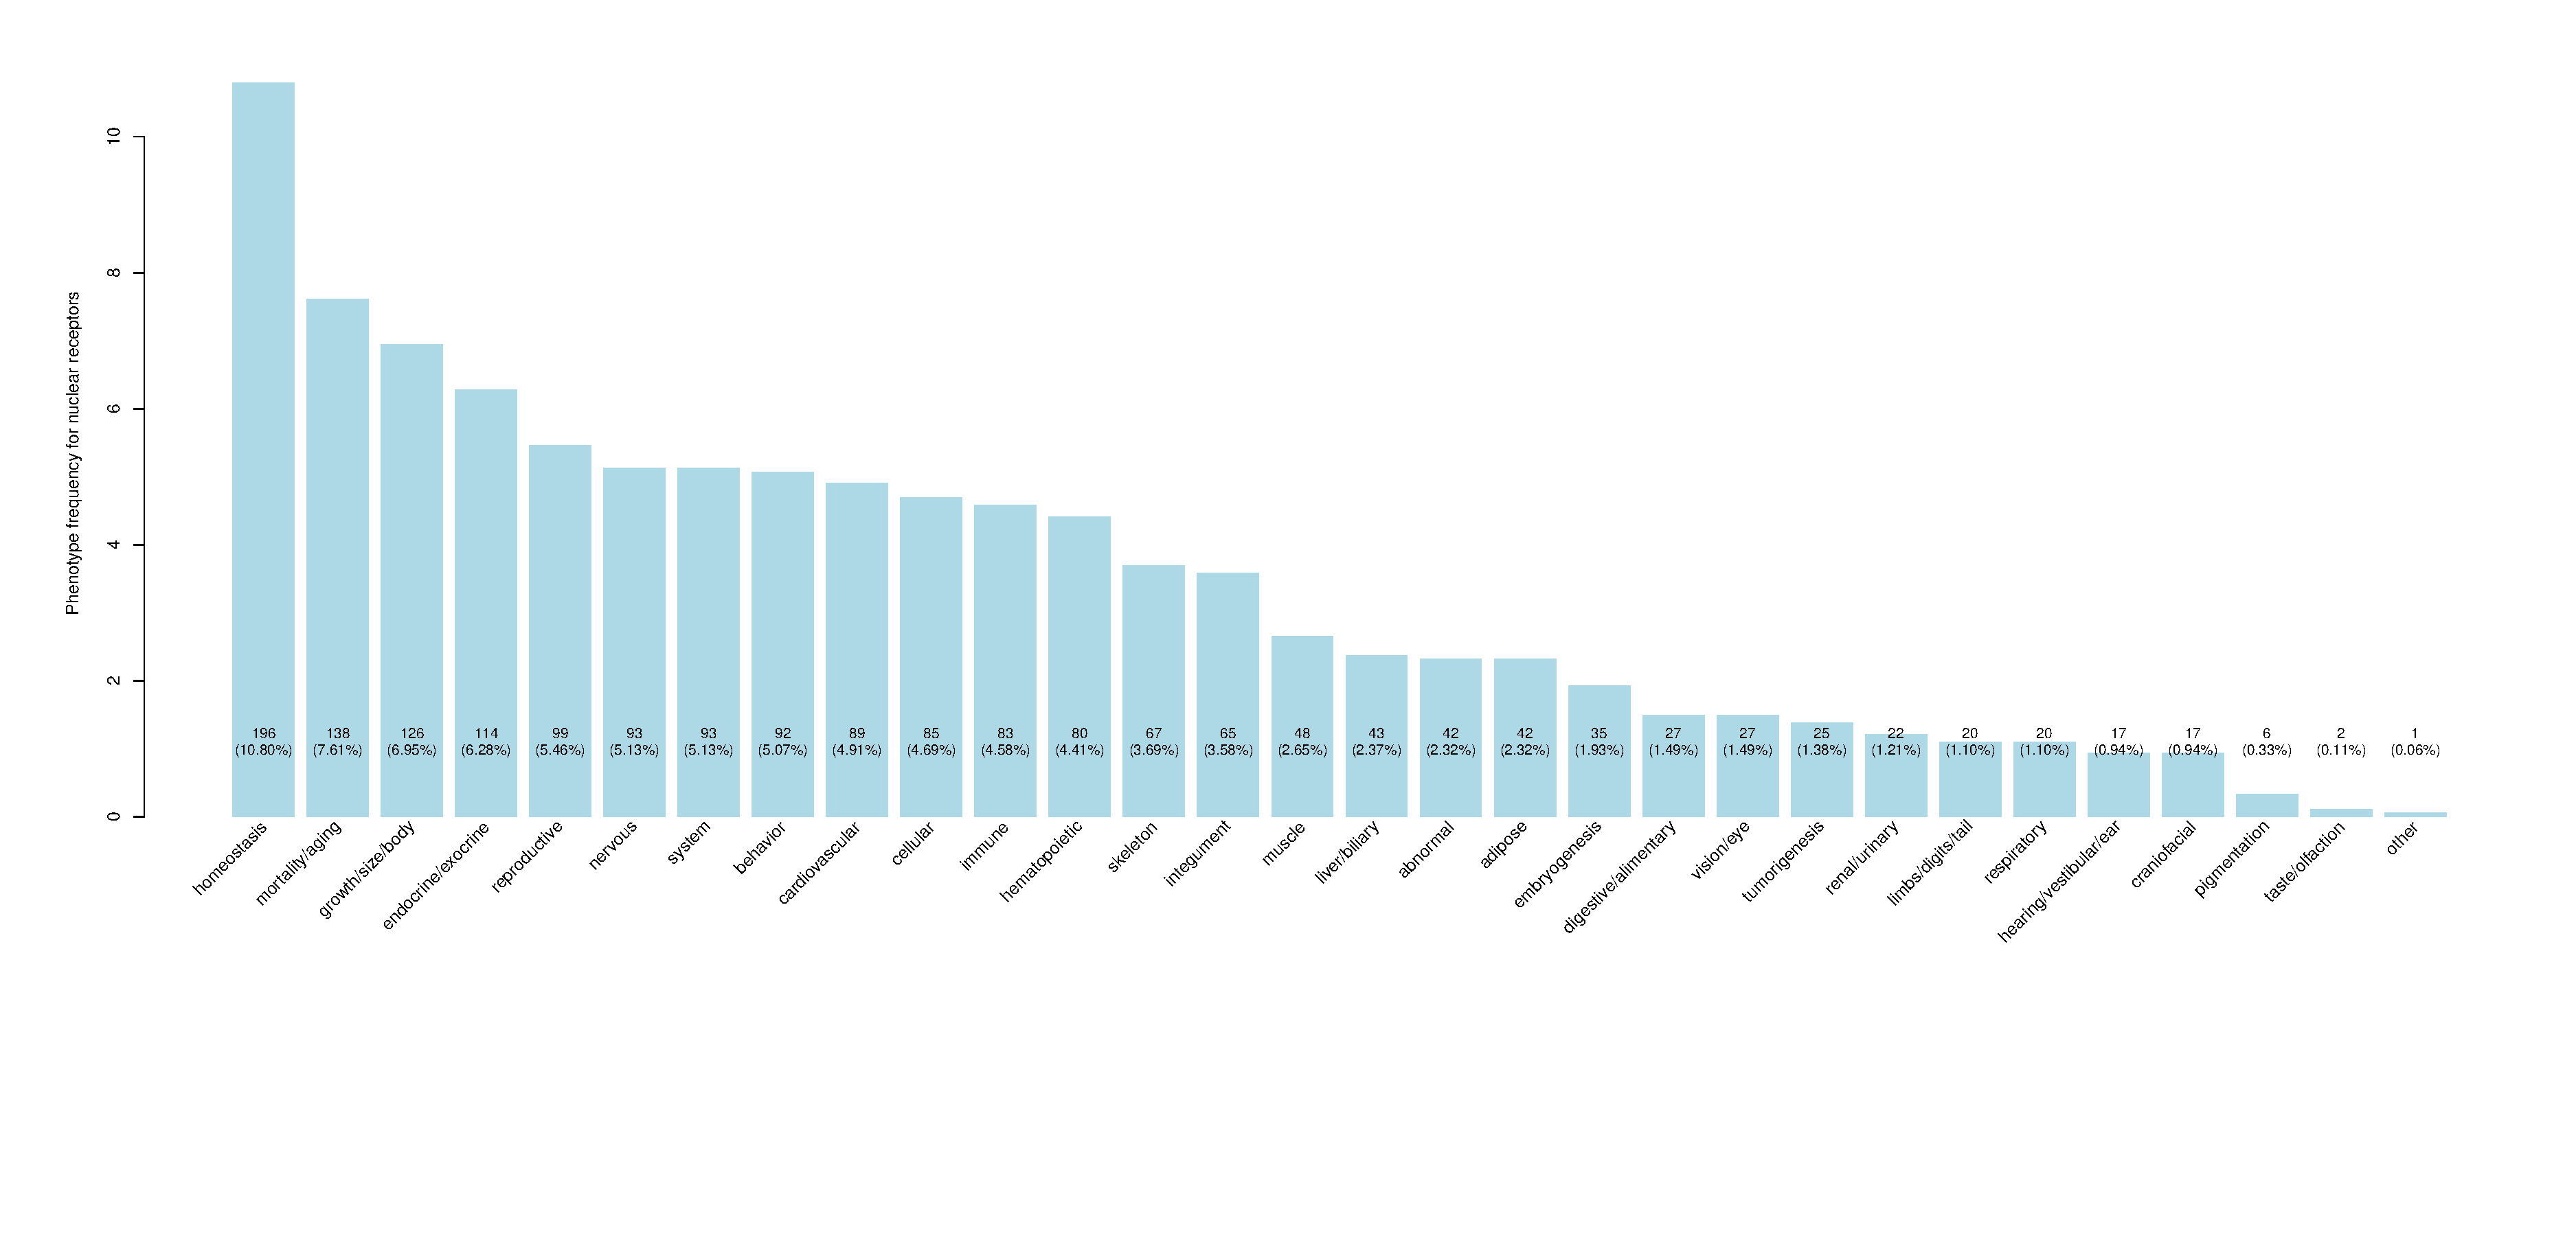
\includegraphics[width=\linewidth]{pics/mgi_phenotypes_distribution.pdf}
	\captionsetup{margin=12pt,format=plain,font=footnotesize,labelfont=bf}
 	\caption{\footnotesize{\textbf{MGI phenotypes}. 
	~~~~~~~\\
	Mouse Genome Informatics phenotype distribution over the genes associated with the 49 nuclear receptors in the mouse.}}
	\label{fig:mgi_pheotypes_distribution}
\end{figure}
~~~~~~~\\
The MGI database consists of generalised definitions of the phenotypes associated with the nuclear receptors found in the mouse. Figure~\ref{fig:mgi_pheotypes_distribution} illustrates the most significant phenotypes and their occurrence frequency across the 242 genes corresponding to the nuclear receptors in the mouse. With a count of 196 matches across the dataset, the most prominent phenotype correlates with the homeostatic metabolic processes, such as temperature regulation and pH-balance. Moreover, Figure~\ref{fig:mgi_pheotypes_nr} provides an insight into the exact association of each phenotype with the corresponding nuclear receptor genes, such that homeostatis, for instance, is prominently found in the following genes: \textit{Esr1}, \textit{Pparg}, \textit{Thrb}, \textit{Thra}, \textit{Vdr} etc. Other phenotypes describe body size and growth features and are representative for the \textit{Pparg} genes.

\begin{figure}[H]
	\centering
	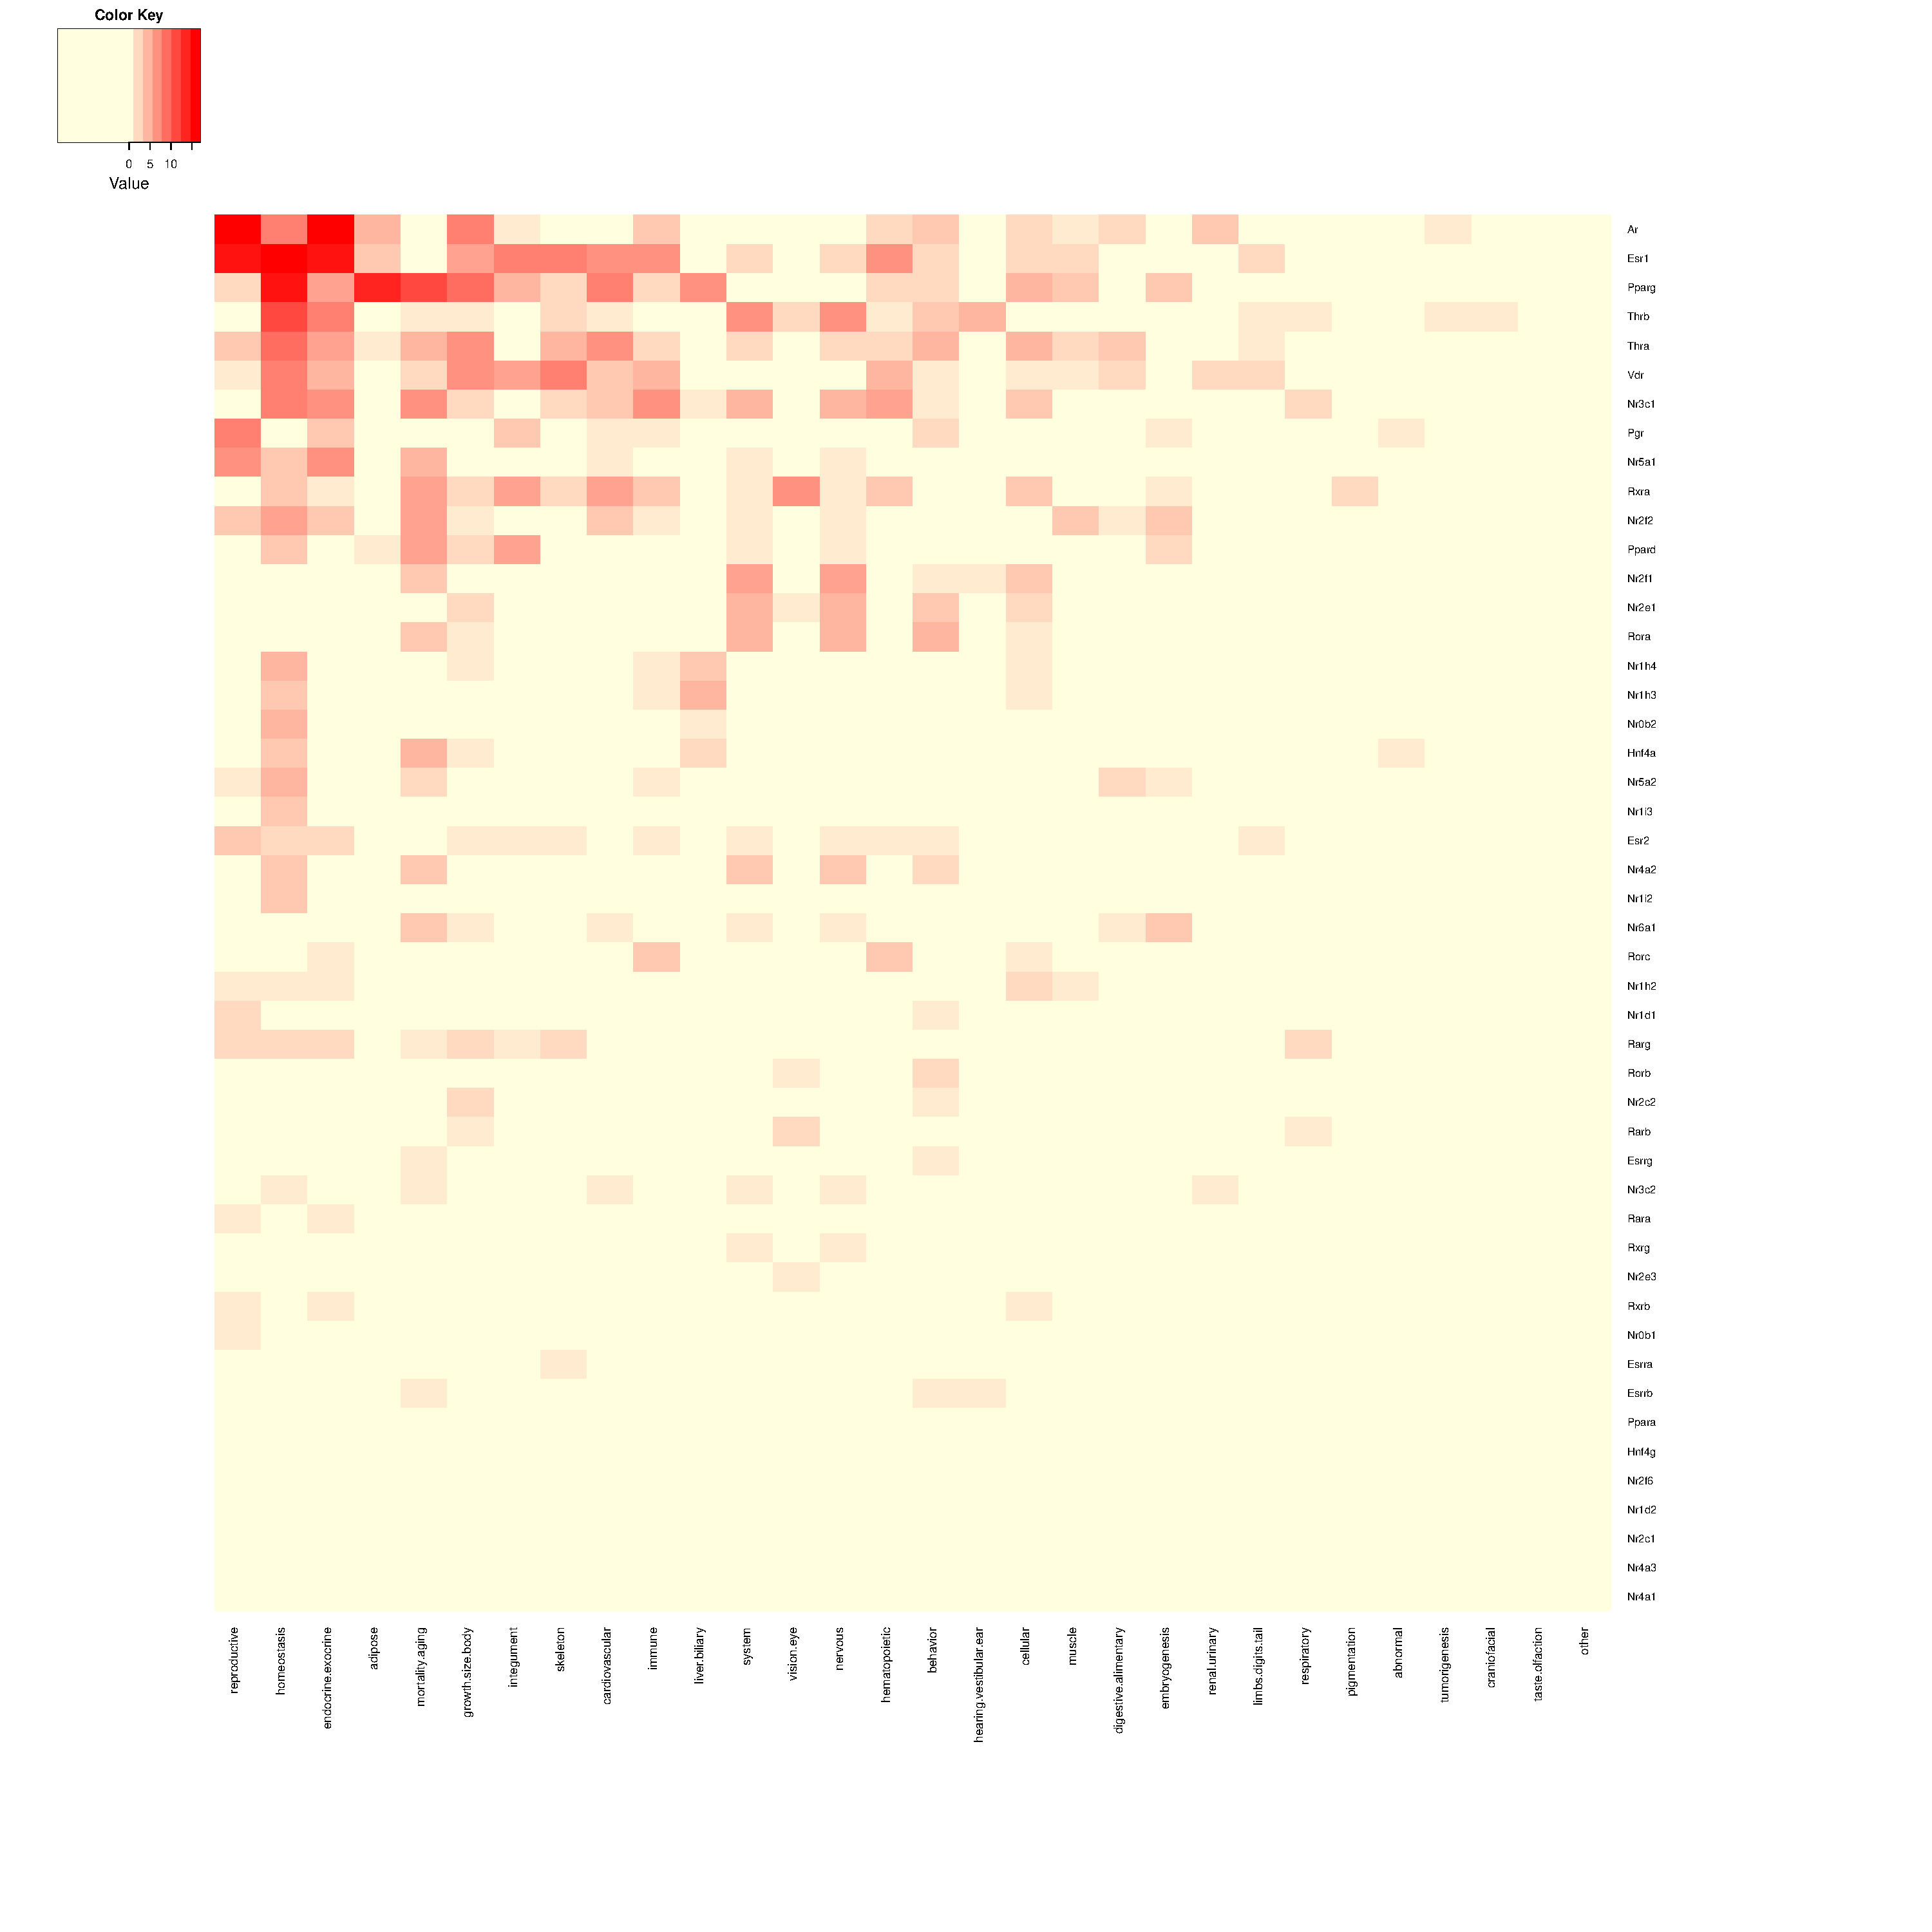
\includegraphics[width=\linewidth, height=0.99\linewidth]{pics/mgi_phenotypes_nr.pdf}
	\captionsetup{margin=12pt,format=plain,font=footnotesize,labelfont=bf}
 	\caption{\footnotesize{\textbf{MGI phenotype - nuclear receptor gene associations}. 
	~~~~~~~\\
	Mouse Genome Informatics phenotype occurrence frequency among the nuclear receptor genes.}}
	\label{fig:mgi_pheotypes_nr}
\end{figure}
~~~~~~~\\

\subsection{MPD Statistics}
\begin{figure}[H]
	\centering
	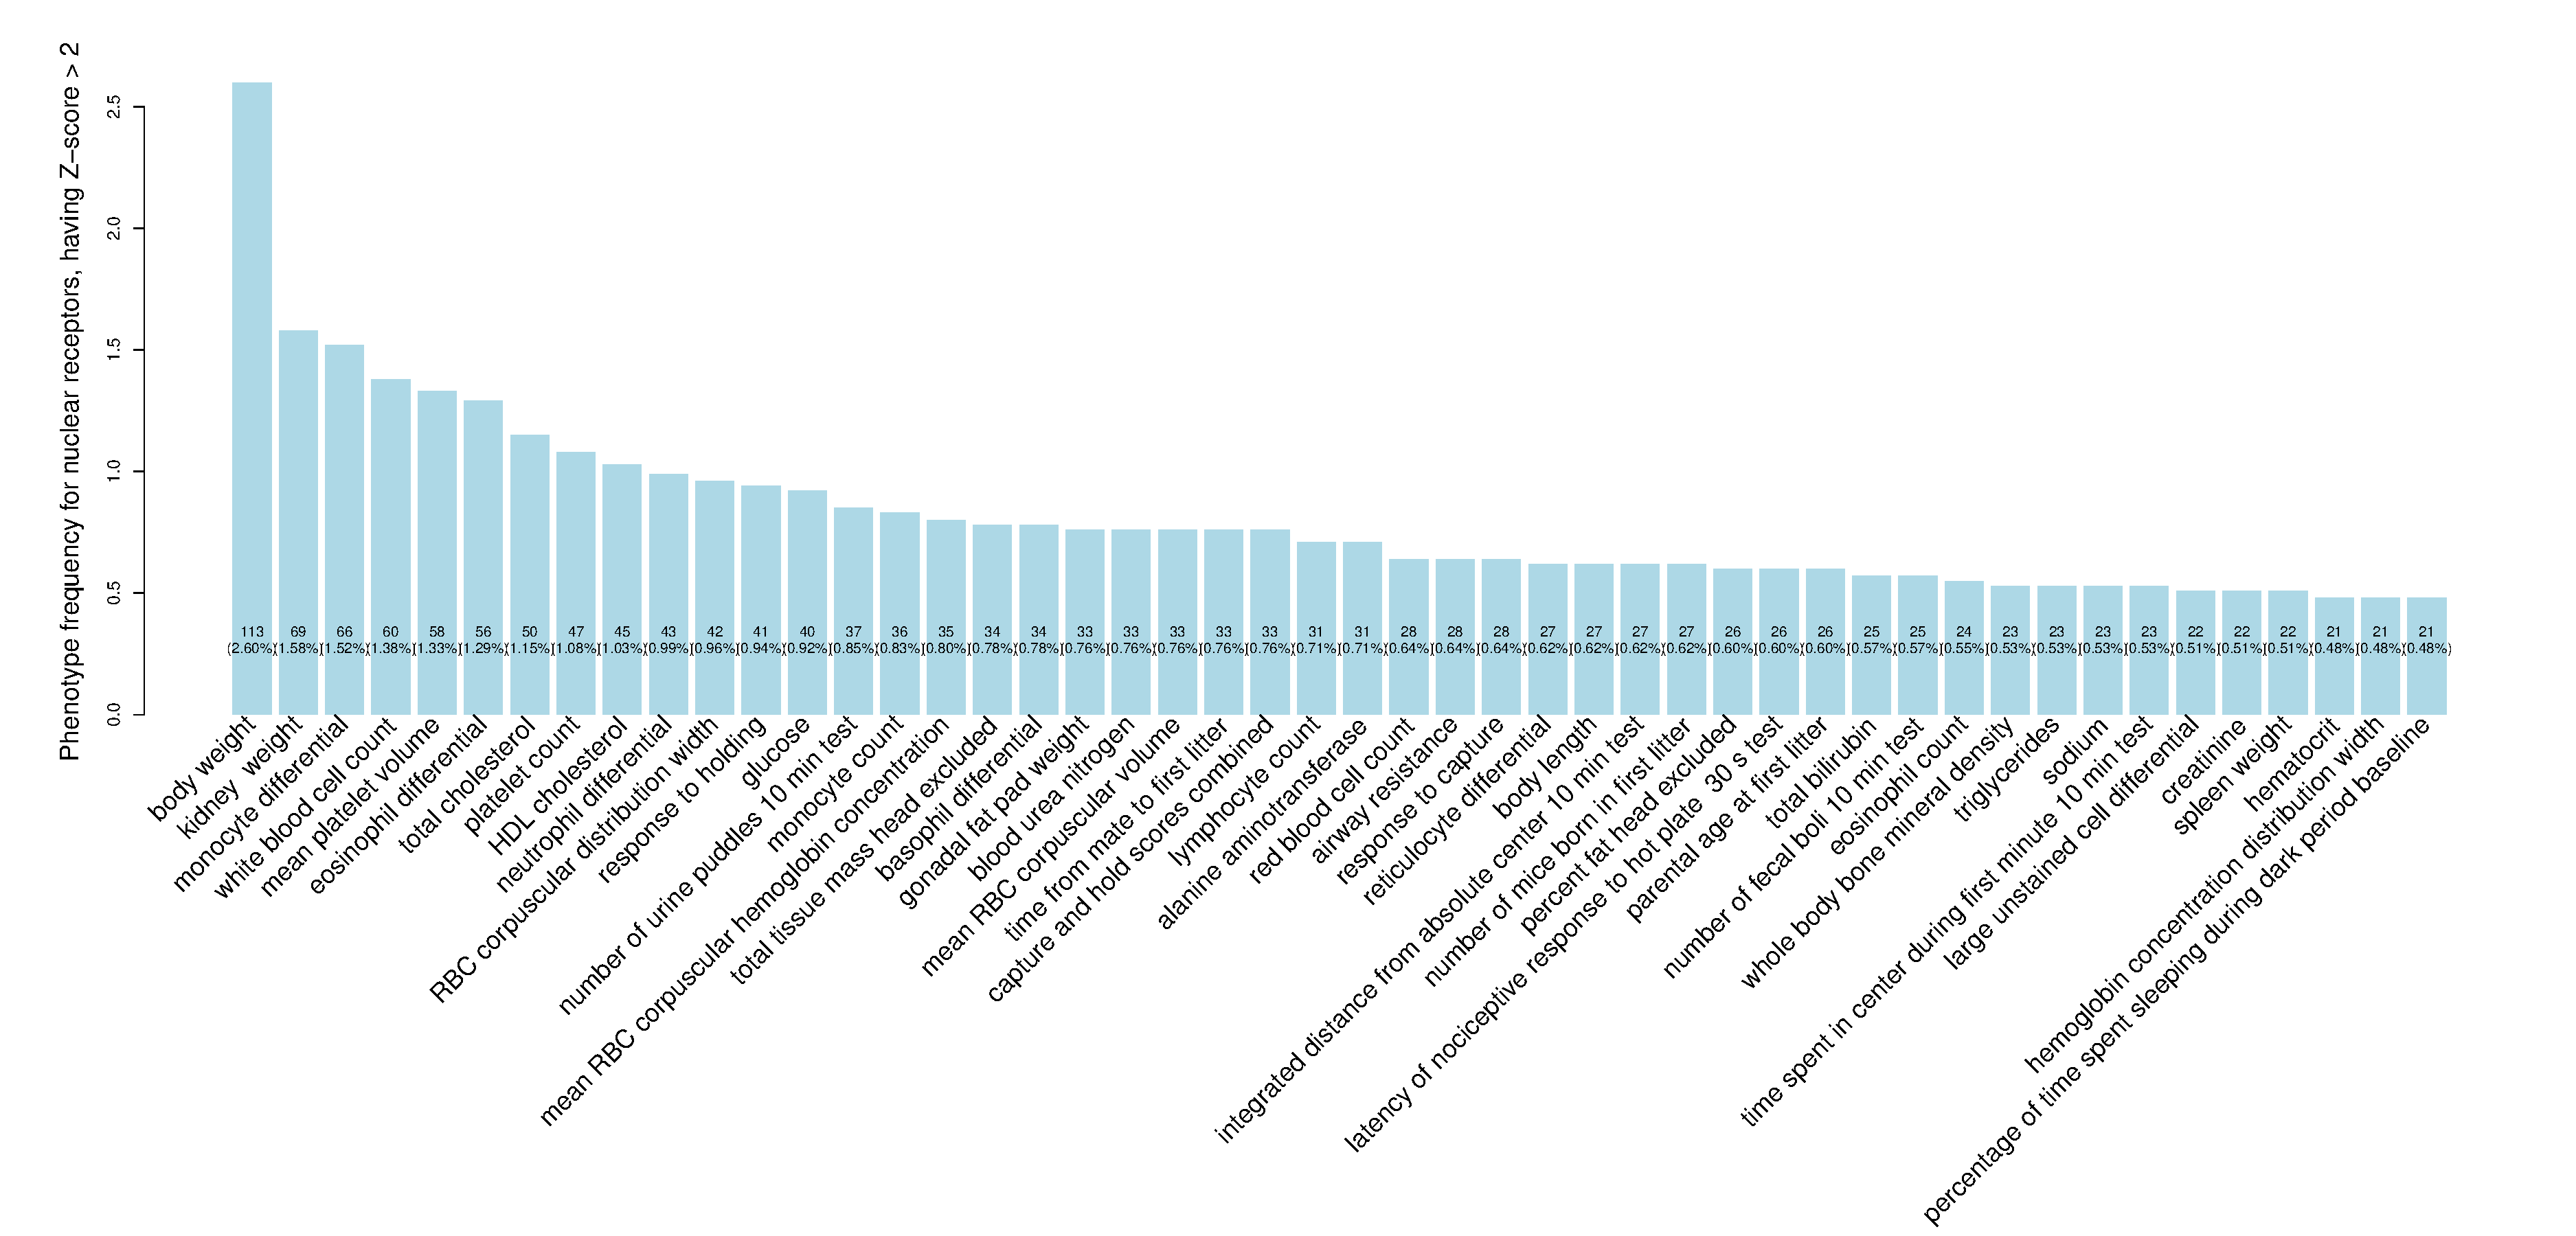
\includegraphics[width=\linewidth]{pics/mpi_phenotypes_distribution_zscore2.pdf}
	\captionsetup{margin=12pt,format=plain,font=footnotesize,labelfont=bf}
 	\caption{\footnotesize{\textbf{MPD phenotypes, having Z-score $>$ 2}. 
	~~~~~~~\\
	Mouse Phenotype Database extreme phenotype distribution over the genes associated with the 49 nuclear receptors in the mouse, having Z-score $>$ 2}}
	\label{fig:mpi_pheotypes_distribution_zscore2}
\end{figure}
~~~~~~~\\

\begin{figure}[H]
	\centering
	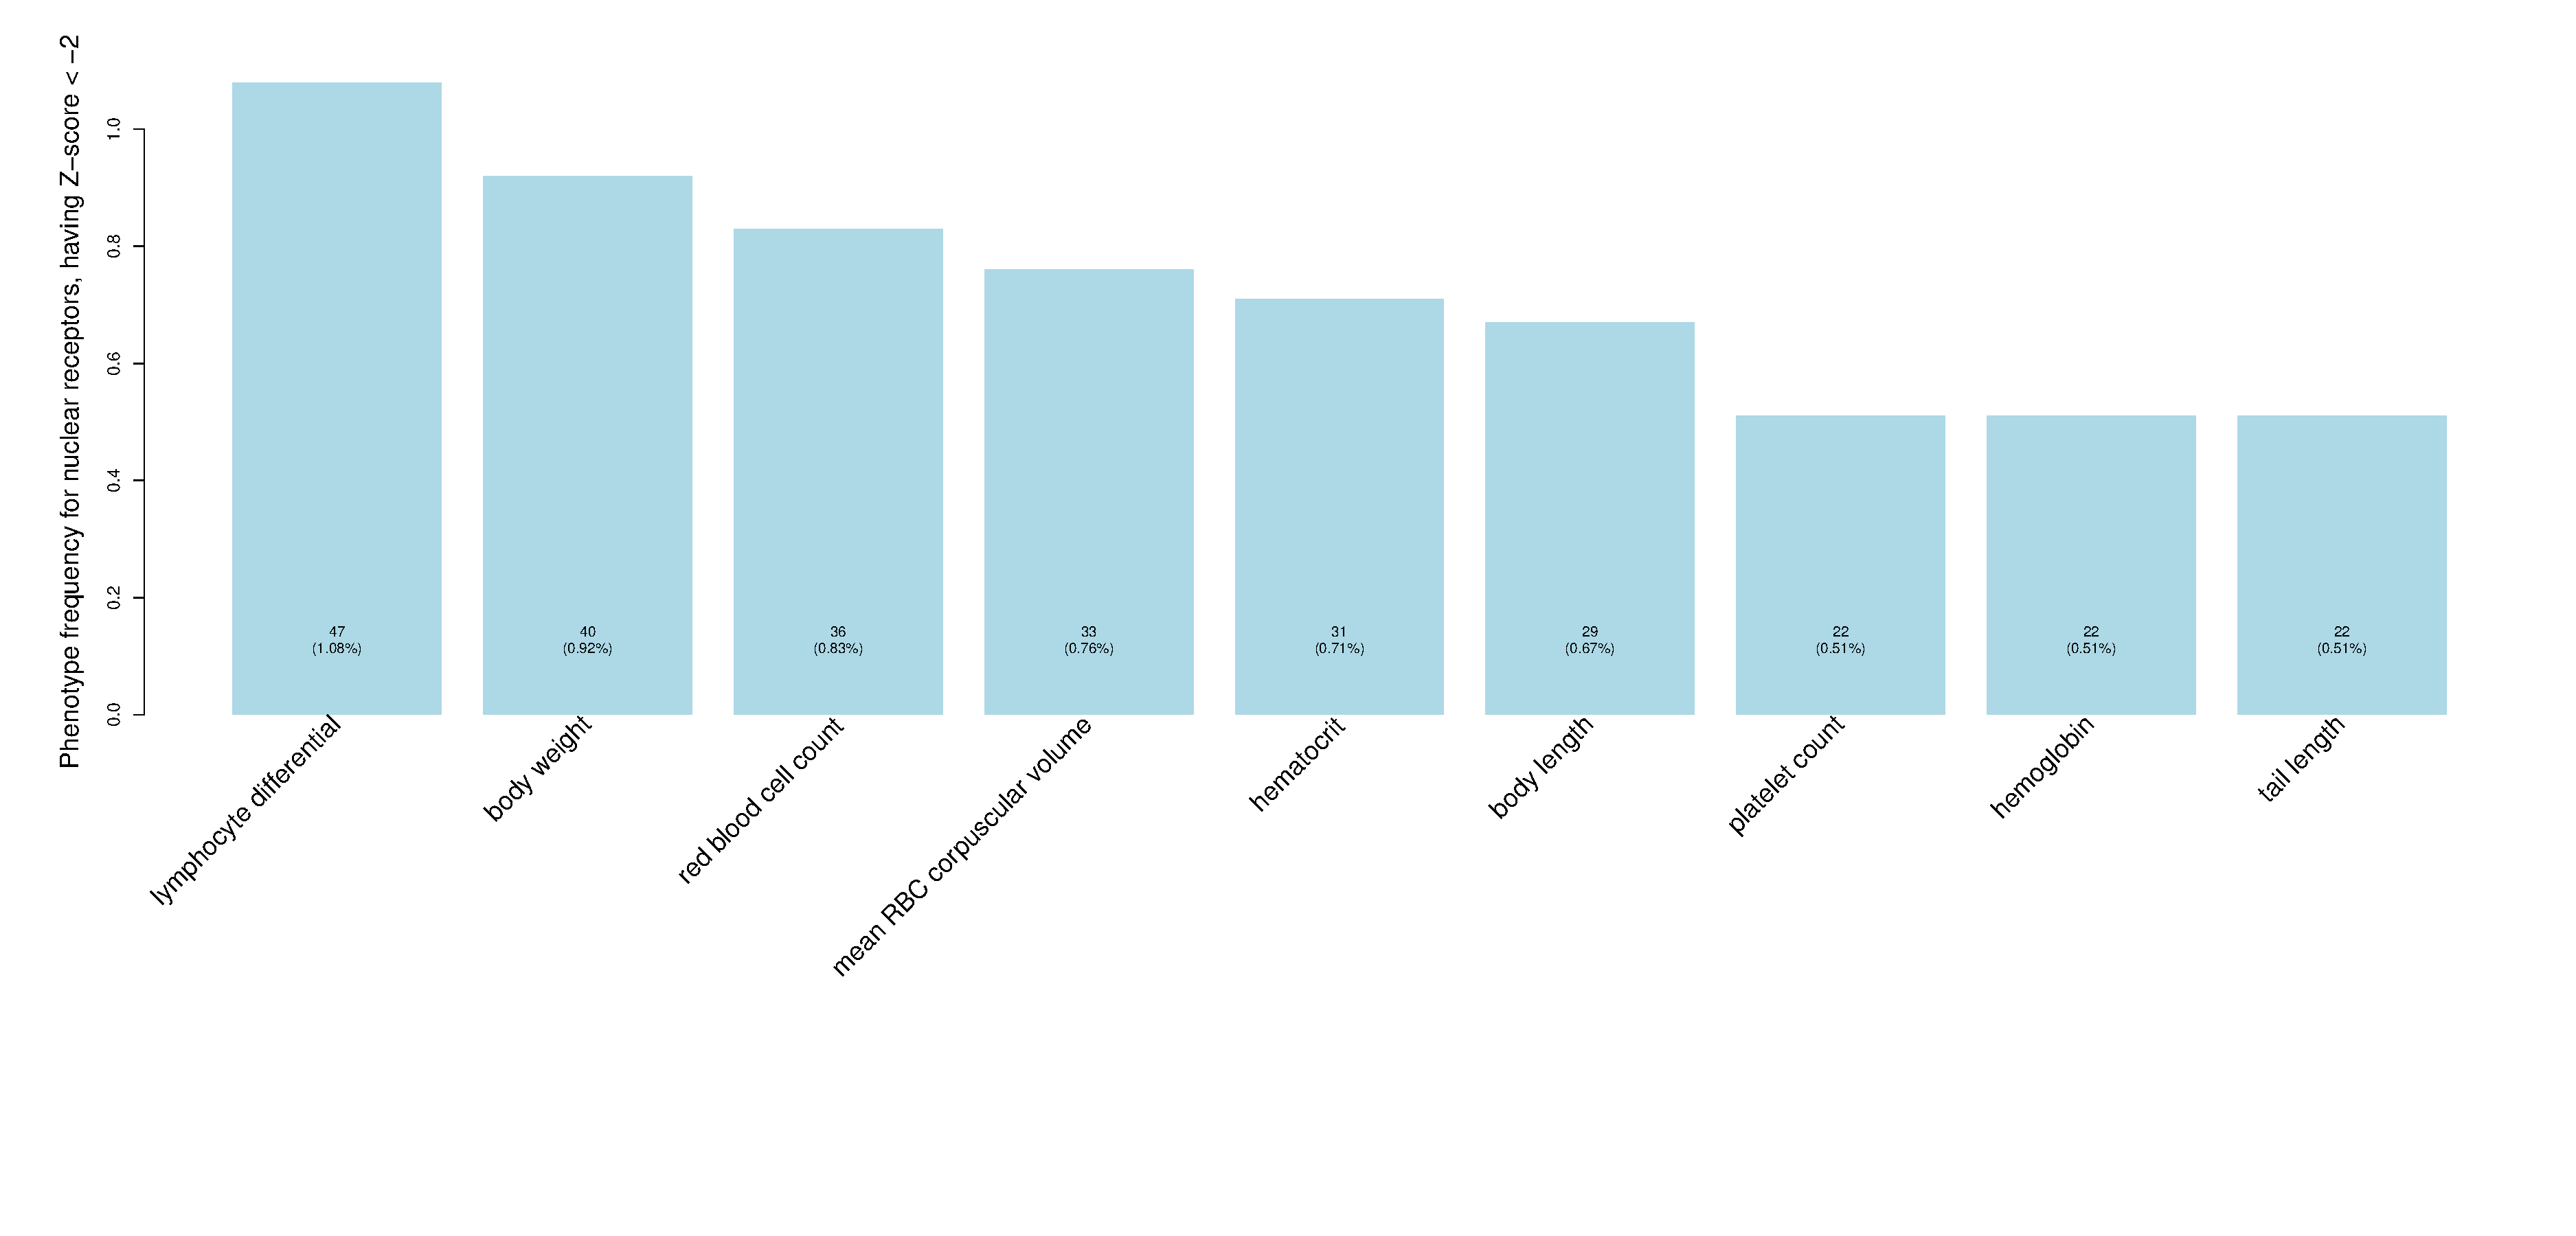
\includegraphics[width=\linewidth]{pics/mpi_phenotypes_distribution_zscore2_neg.pdf}
	\captionsetup{margin=12pt,format=plain,font=footnotesize,labelfont=bf}
 	\caption{\footnotesize{\textbf{MPD phenotypes, having Z-score $<$ -2}. 
	~~~~~~~\\
	Mouse Phenotype Database extreme phenotype distribution over the genes associated with the 49 nuclear receptors in the mouse, having Z-score $<$ -2}}
	\label{fig:mpi_pheotypes_distribution_zscore2_neg}
\end{figure}
~~~~~~~\\
~~~~~~~\\
The MPDatabase contains annotations for extreme phenotypes associated with different mouse strains. An extreme phenotype is described by a Z-score above 2 (very high) or below -2 (very low), relative to other measurement means. Based on these specifications, Figure~\ref{fig:mpi_pheotypes_distribution_zscore2} illustrates the most significant phenotypes and their occurrence frequency across the 242 genes corresponding to the nuclear receptors in the mouse, with a Z-score $>$ 2 (extreme high phenotypes). Here, the most significant phenotypes include \textit{body weight}, \textit{kidney weight} and \textit{cholesterol}. Similarly, Figure~\ref{fig:mpi_pheotypes_distribution_zscore2_neg} presents the most significant phenotypes and their occurrence frequency across the 242 genes corresponding to the nuclear receptors in the mouse, having a Z-score $<$ -2 (extreme low phenotypes). In this case, the most significant phenotypes include \textit{body weight} as well, but the focus lies on several blood phenotypes (e.g. lymphocyte differential, red blood cell count, hemoglobin). 
~~~~~~~\\
~~~~~~~\\
Table~\ref{tab:top10pheno} shows the strains and gene names associated with the most significant MPD phenotypes. 
\begin{table}[H]
\centering
\begin{tabulary}{\linewidth}{ LLLLL }
\hline
	\textbf{Strain} & \textbf{Gene}  & \textbf{Phenotype} & \textbf{Z-score}
	\\  
	\hline \hline 
	CAST/EiJ  & Rora (RAR-related orphan receptor alpha) & trigonelline relative abundance &  8.8 \\
	C58/J  & Rorc (RAR-related orphan receptor gamma) & N-acetylglutamate relative abundance & 8.4\\ 
	CAST/EiJ  & Rara (retinoic acid receptor, alpha) & N2-acetyllysine (16h fast), relative abundance &  4.6\\ 
	NZB/BlNJ & Nr1i3 (nuclear receptor subfamily 1, group I, member 3) & ECG parameters interval between peak of P-wave to R-wave (PR) &  4.6\\ 
	CE/J & Nr0b1 (nuclear receptor subfamily 0, group B, member 1) & kidney total weight &  4.4\\
	NZB/BlNJ  & Nr5a1 (nuclear receptor subfamily 5, group A, member 1) & succinylcarnitine relative abundance  &  3.8\\
	C57L/J & Esr2 (estrogen receptor 2 beta) & 
	relative size of perivascular immune cell clusters &  3.5\\
	NOD/\\ShiLtJ & Ppard (peroxisome proliferator activator receptor delta) & 
	percentage of parasites in brain relative to all organs tested &  3.1\\ 
	BUB/BnJ & Esr1 (estrogen receptor 1 alpha) & 3-dehydrocarnitine  relative abundance &  2.7\\  
	\hline
\end{tabulary}
\caption{\footnotesize{\textbf{Top 10 extreme phenotypes.} 
~~~~~~~\\
Mouse strains associated with extreme phenotypes, based on their Z-score.}} 
\label{tab:top10pheno}
\end{table}
~~~~~~~\\
Moreover, Figures~\ref{fig:mpi_pheotypes_strain_zscore2} and~\ref{fig:mpi_pheotypes_strain_zscore2_neg} provide an insight into the exact association of each phenotype with the corresponding nuclear receptor genes. Therefore, there are ... genes associated with the extreme high phenotypes and 5 genes associated with the extreme low phenotypes, respectively, as following: \textit{Rora}, \textit{Esr1}, \textit{Esrrg}, \textit{Thrb} and \textit{Nr3c2}. 
\begin{figure}[H]
	\centering
	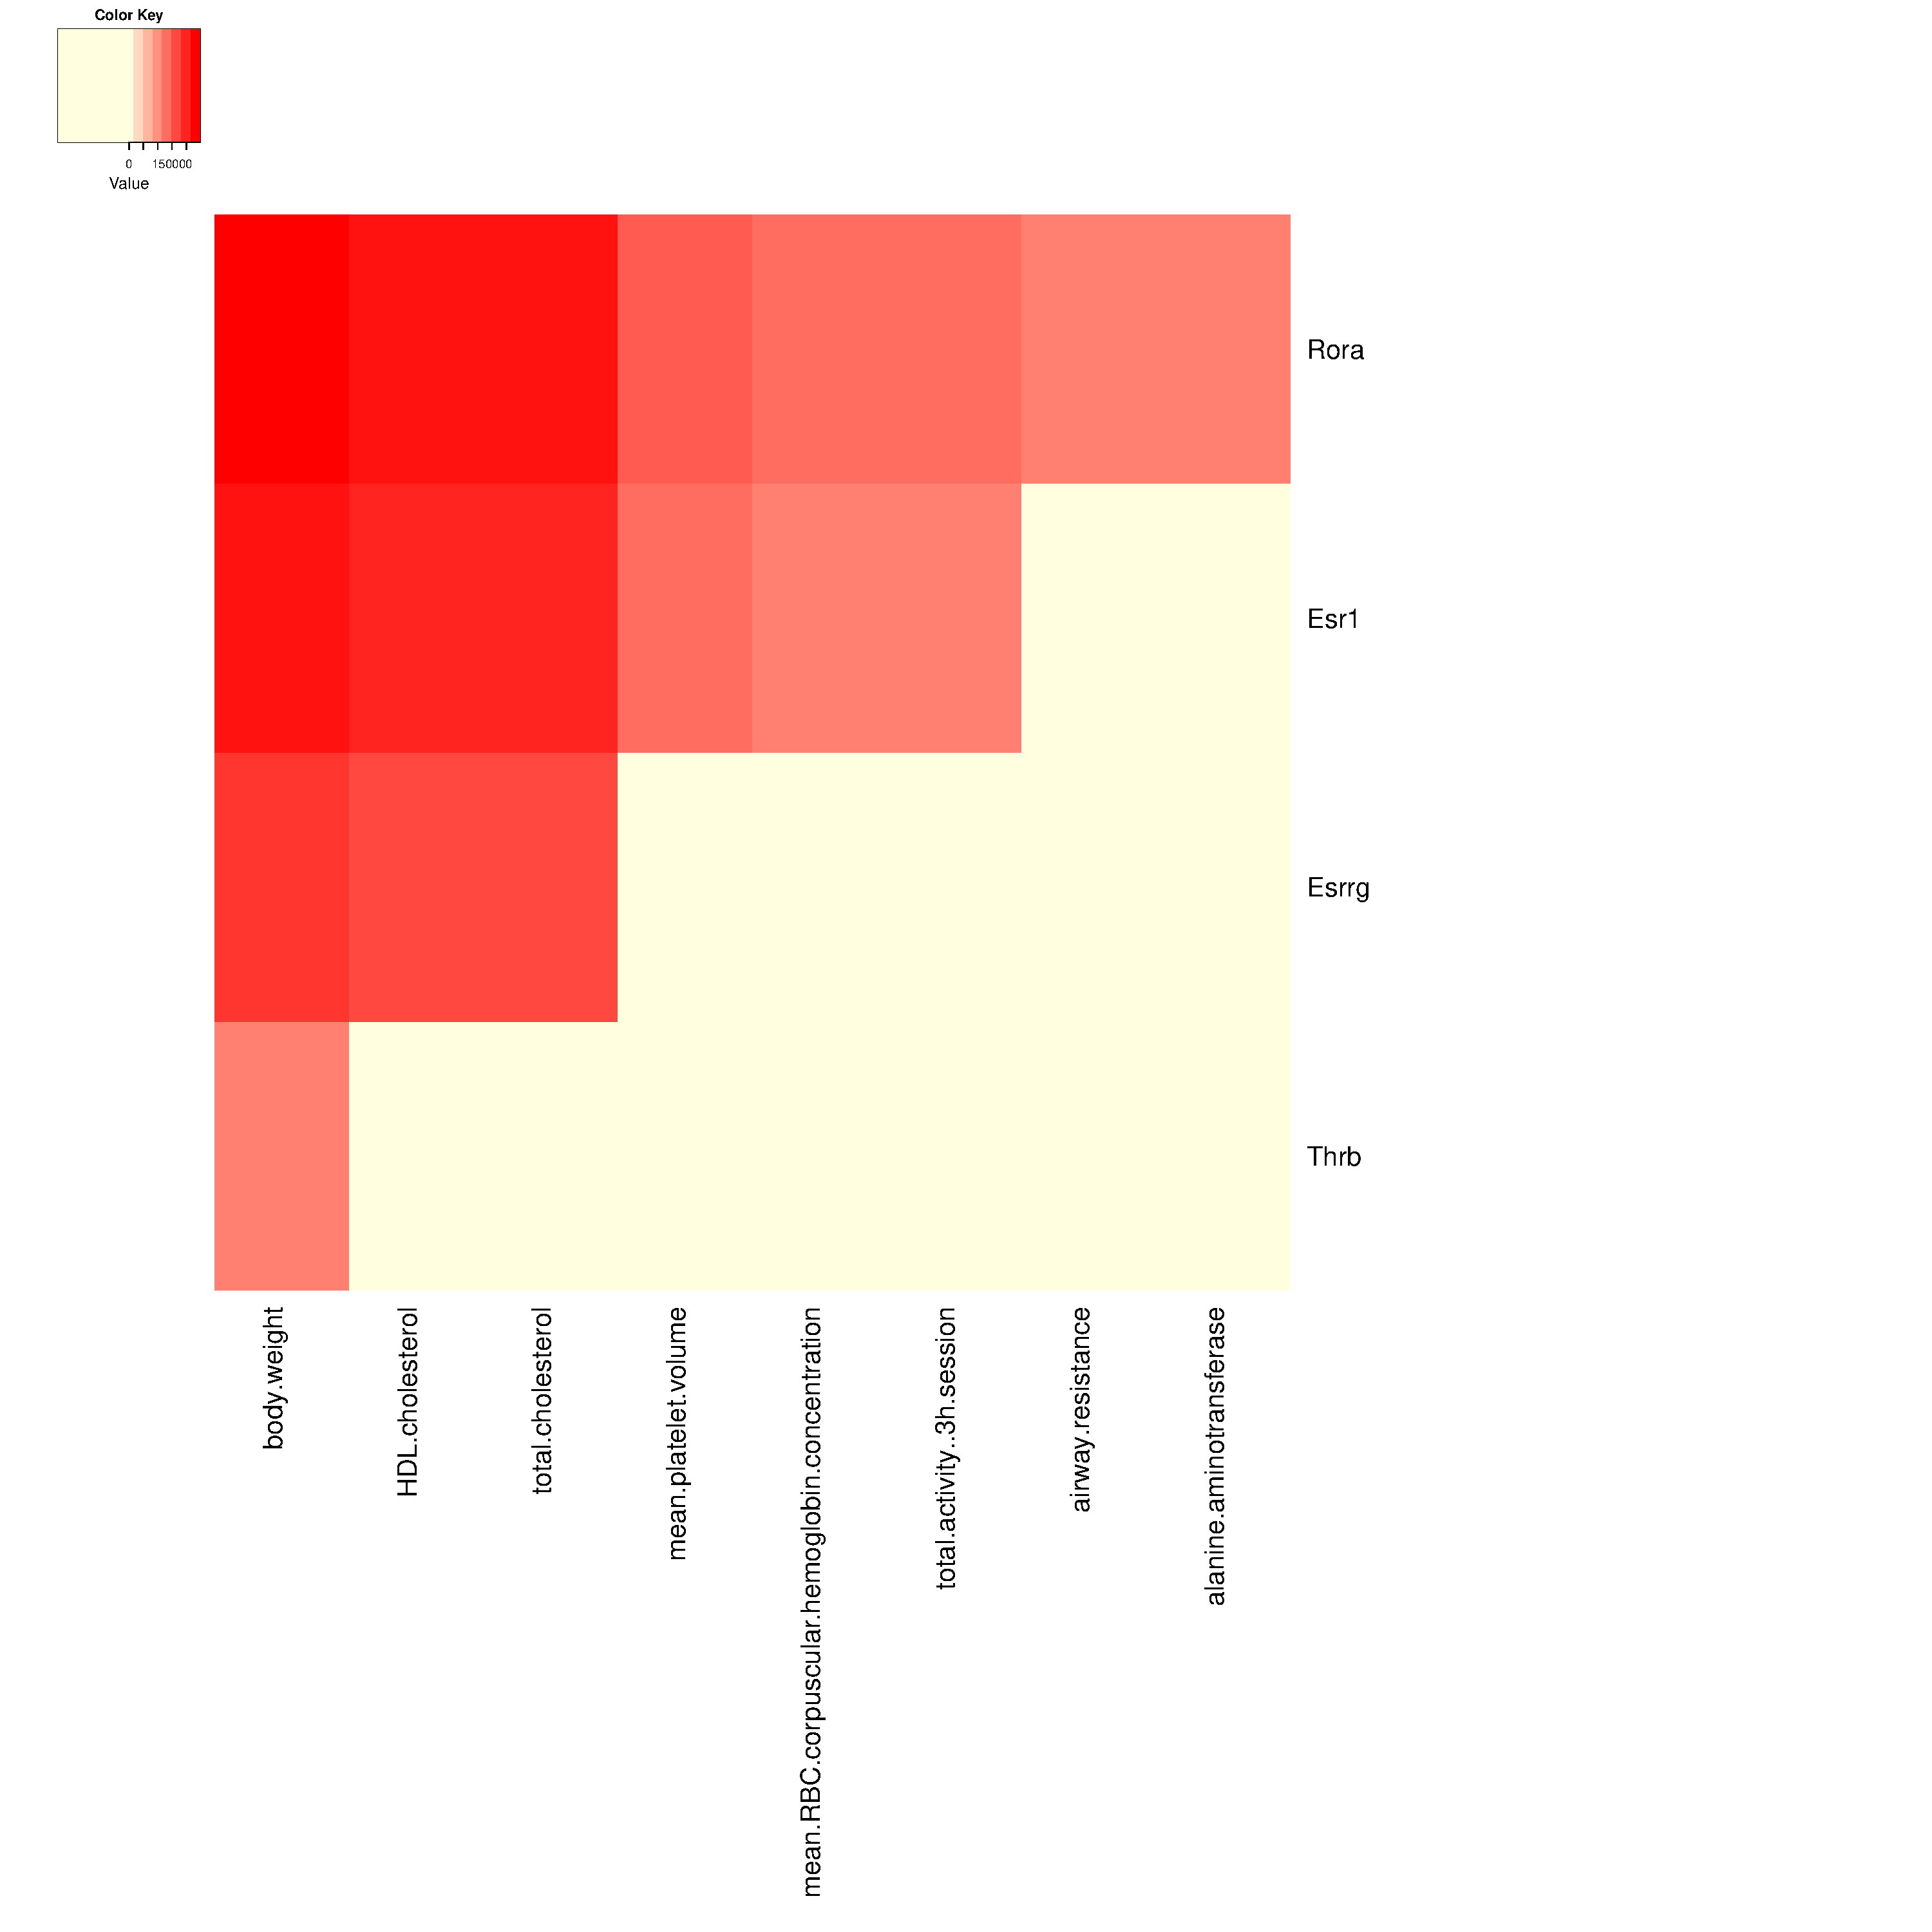
\includegraphics[width=\linewidth]{pics/mpi_phenotypes_nr_zscore2.pdf}
	\captionsetup{margin=12pt,format=plain,font=footnotesize,labelfont=bf}
 	\caption{\footnotesize{\textbf{MPD extreme phenotypes, having Z-score $>$ 2}. 
	~~~~~~~\\
	Mouse Phenome Database extreme phenotype occurrence frequency among the 49 nuclear receptors in the mouse, having Z-score $>$ 2}}
	\label{fig:mpi_pheotypes_strain_zscore2}
\end{figure}
~~~~~~~\\

\begin{figure}[H]
	\centering
	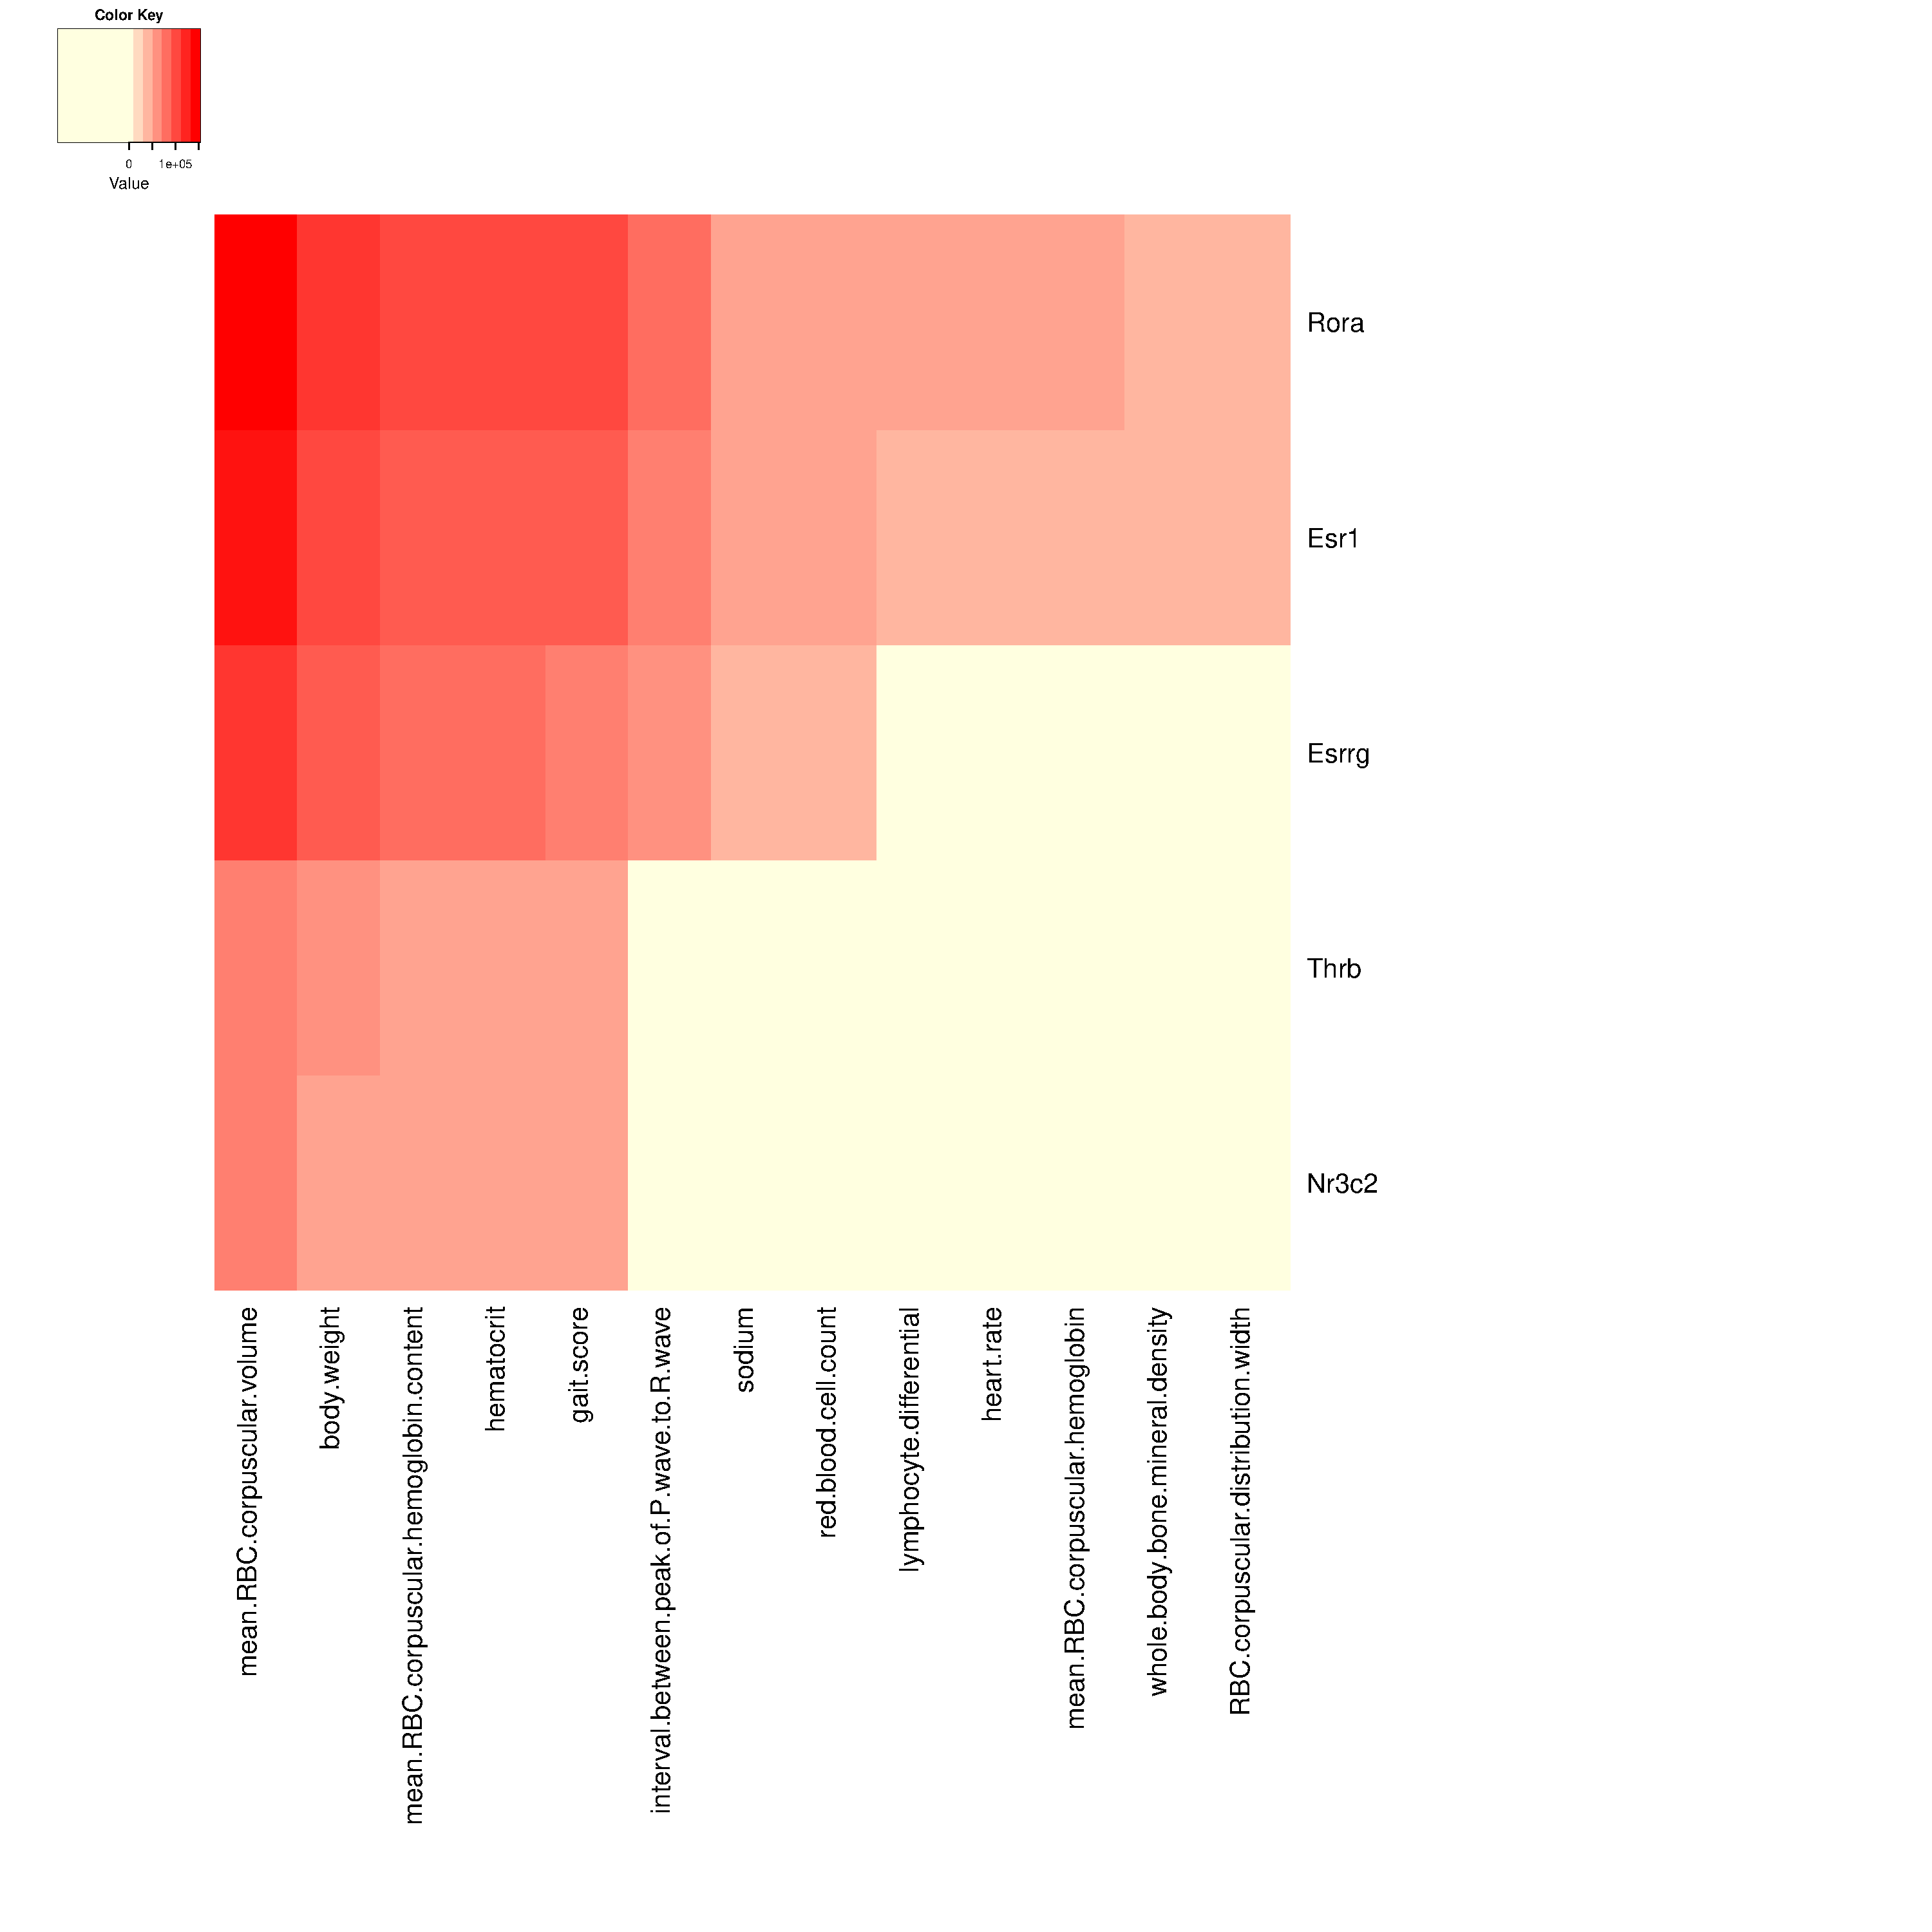
\includegraphics[width=\linewidth]{pics/mpi_phenotypes_nr_zscore2_neg.pdf}
	\captionsetup{margin=12pt,format=plain,font=footnotesize,labelfont=bf}
 	\caption{\footnotesize{\textbf{MPD extreme phenotypes, having Z-score $<$ -2}. 
	~~~~~~~\\
	Mouse Phenome Database extreme phenotype occurrence frequency among the 49 nuclear receptors in the mouse, having Z-score $<$ -2}}
	\label{fig:mpi_pheotypes_strain_zscore2_neg}
\end{figure}
~~~~~~~\\

%------------------------------------------------
\section{Discussion and Outlook}

Blabla 

%------------------------------------------------
\section{Acknowledgments} % The \section*{} command stops section numbering

Our gratitude to Prof. Dr. H. W. Mewes for offering us the topic and the opportunity to work with the Helmholz Zentrum research centre in Munich. Many thanks to our supervisor, Dr. Desislava Boyanova for all the input and ideas, discussions, advices and foremost her useful and critical suggestions which motivated us a lot. Last but not least, we would like to thank our fellow colleagues for their support, as well as the entire \emph{Helmholz Zentrum} group. 
%----------------------------------------------------------------------------------------
% Appendix
%----------------------------------------------------------------------------------------
\section{Appendix}
\label{an:appendix}
List of gene names associated with the 49 mouse nuclear receptors:
~~~~~~~\\
~~~~~~~\\
\textit{Esrrg, Rorc, Nr1i2, Hnf4g, Nr0b1, Nr3c1, Hnf4a, Rxrg, Esrra, Thrb, Nr5a1, Pparg, Nr4a1, Nr5a2, Nr1h3, Nr4a3, Nr1i3, Nr2f2, Nr4a2, Nr2f6, Esrrb, Ppard, Nr2e1, Vdr, Nr6a1, Nr1h5, Rarb, Nr1h2, Esr1, Rora, Rarg, Nr1h4, Rara, Nr3c2, Pgr, Ar, Rxrb, Thra, Esr2, Rorb, Ppara, Nr1d1, Nr0b2, Nr2e3, Nr2f1, Nr1d2, Nr2c1, Rxra, Nr2c2}.

%----------------------------------------------------------------------------------------
%	REFERENCE LIST
%----------------------------------------------------------------------------------------
\phantomsection
\bibliographystyle{unsrt}
\bibliography{sample}

%----------------------------------------------------------------------------------------

\end{document}